\documentclass[12pt]{beamer}
\usepackage{silence}
\WarningFilter{beamerthememetropolis}{You need to compile with XeLaTeX or LuaL
aTeX to use the Fira fonts}
\WarningFilter{biblatex}{Patching footnotes failed.}

\usepackage{fixltx2e}
\usepackage[T1]{fontenc}
\usepackage{lmodern}
\usepackage[lining, sfdefault, scaled=.88]{FiraSans}
\usepackage{newtxsf}
\usetheme[block=fill]{metropolis}
%These are Metropolis' core colours
%\definecolor{mDarkBrown}{HTML}{604c38}
%\definecolor{mDarkTeal}{HTML}{23373b}
\definecolor{mLightBrown}{HTML}{E83D0C}
%\definecolor{mLightGreen}{HTML}{14B03D}
\setbeamerfont{alerted text}{series=\bfseries}
\usepackage[bb=fourier]{mathalfa}
\let\inside\subseteq
\newcommand\reals{\mathbb R}
\usepackage{mathtools}
\DeclarePairedDelimiter{\setof}{\{\,}{\,\}}

\usepackage[backend=biber]{biblatex}
\addbibresource{fractals.bib}
\usepackage{array} 
\usepackage{booktabs}
\usepackage{xfrac}
\usepackage{xcolor}
\usepackage{newtxsf}

\title{A spotter's guide to fractals}
\subtitle{What, Why and How}
\author{David Robertson}
\date{Wednesday 16\textsuperscript{th} November 2016}

\newcommand\dimT{\operatorname{dim}_{\operatorname{Top}}}
\newcommand\dimB{\operatorname{dim}_{\operatorname{Box}}}
\newcommand\dimS{\operatorname{dim}_{\operatorname{Sim}}}

%TikZ gibberish
\def\kochsegment#1#2{--++(#1:#2) -- ++(#1+60:#2) -- ++(#1-60:#2) -- ++(#1:#2)}
%http://tex.stackexchange.com/a/146991/82389
\tikzset{
    invisible/.style={opacity=0,text opacity=0},
    visible on/.style={alt={#1{}{invisible}}},
    alt/.code args={<#1>#2#3}{%
      \alt<#1>{\pgfkeysalso{#2}}{\pgfkeysalso{#3}} % \pgfkeysalso doesn't change the path
    },
    alert on/.style={alt={#1{red}{}}}
  }

\newcommand\picframe[2]{
	{
	\setbeamertemplate{background canvas}{
		\includegraphics[height=\paperheight, keepaspectratio]{#1}
	}
	\begin{frame}[standout]
		\frametitle{\mbox{#2}}
	\end{frame}
	}
}

\begin{document}
\pagestyle{empty}
\begin{frame}
\titlepage
\end{frame}

\section{WHAT: real world examples}

\foreach \desc/\name in {%
	Clouds are not spheres/clouds,
	Mountains are not cones/mountains,
	Coastlines are not circles/coastline,
	Bark is not smooth/bark,
	Lightning doesn't travel in a straight line/lightning} {
	\picframe{../media/\name}{\desc}
}

\begin{frame}
\vspace{1cm}
\begin{tabular}{m{0.45\linewidth}m{0.45\linewidth}l}
	 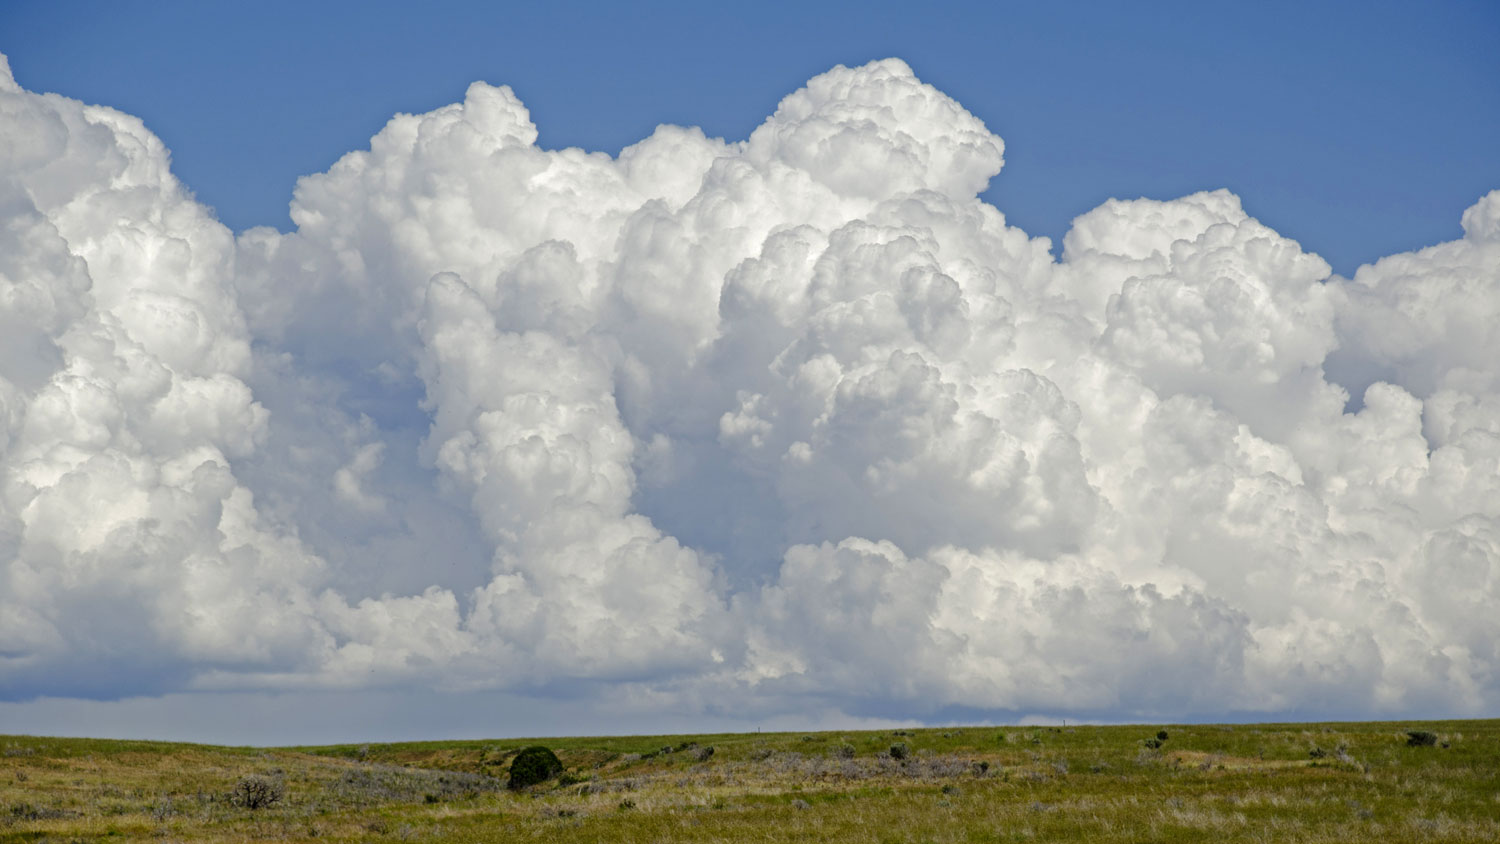
\includegraphics[width=\linewidth, height=0.25\paperheight]{../media/clouds}
	&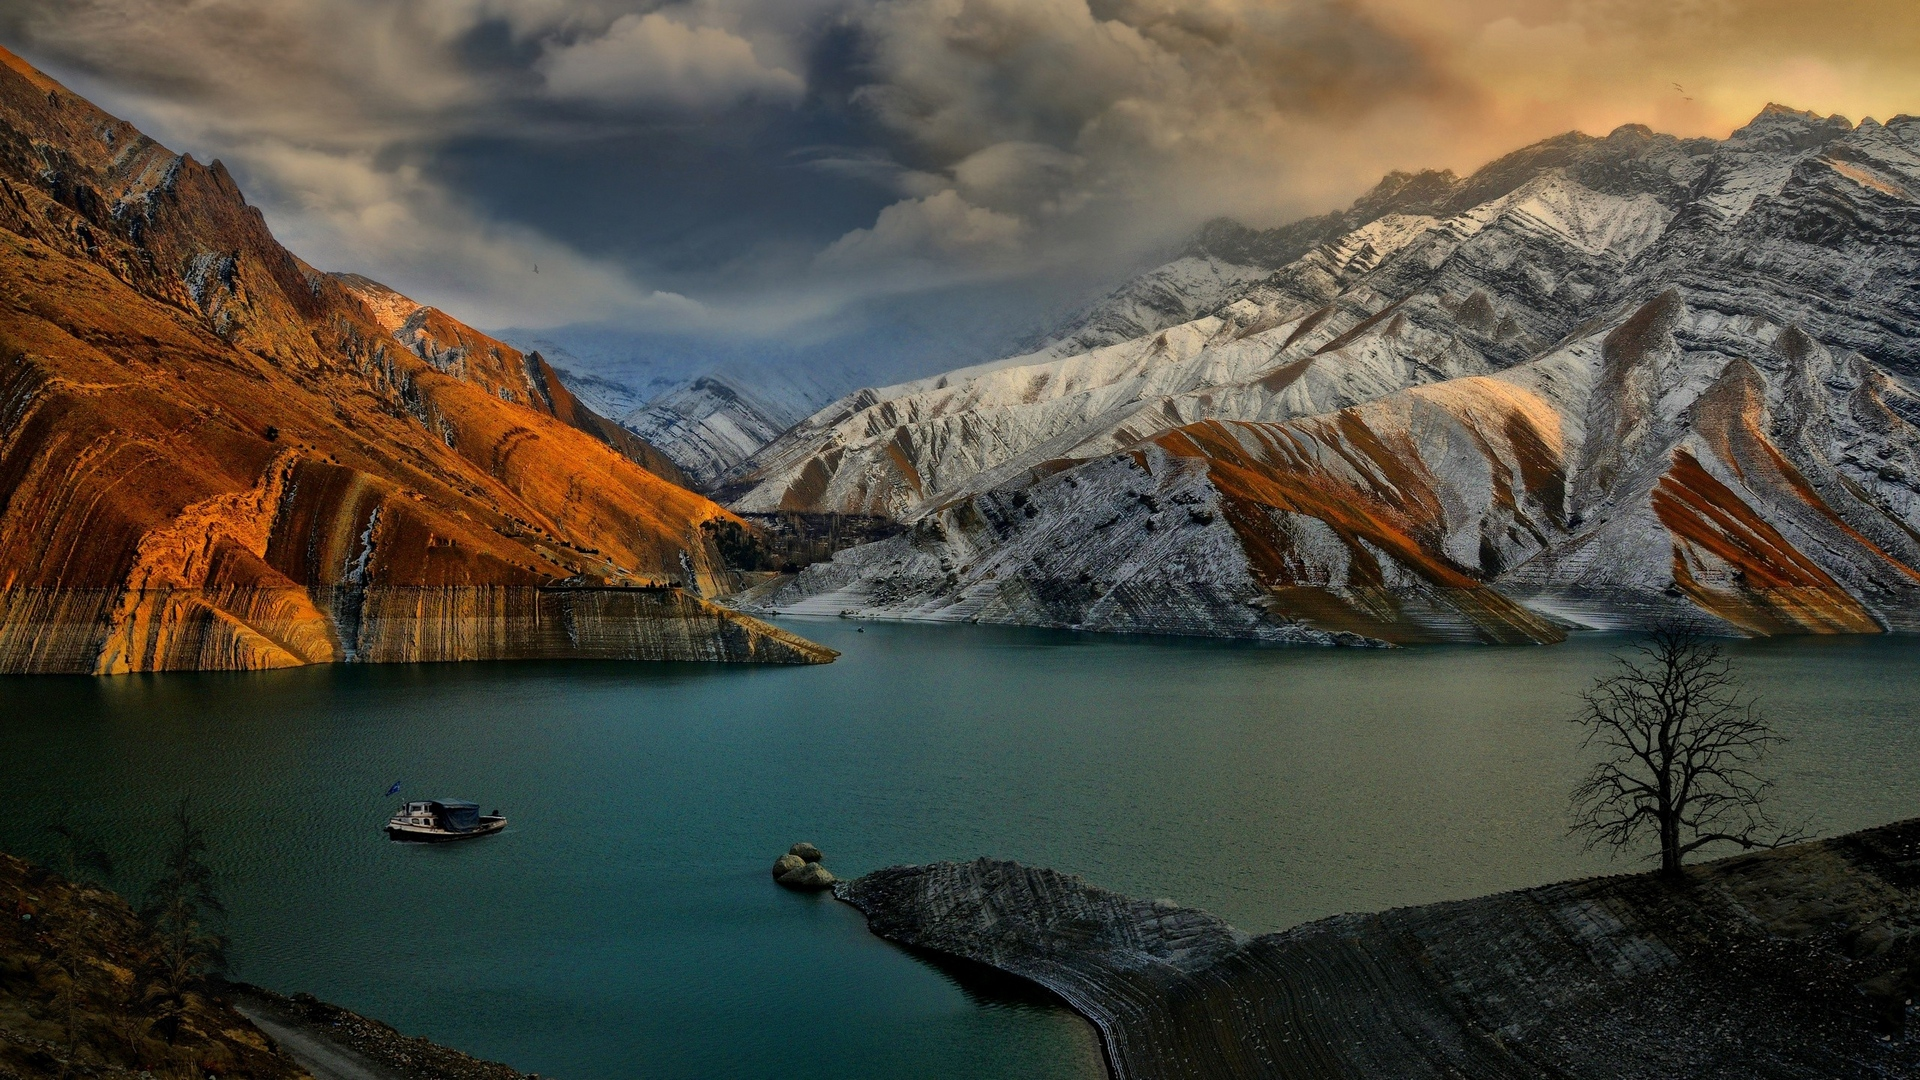
\includegraphics[width=\linewidth, height=0.25\paperheight]{../media/mountains} &\\
	 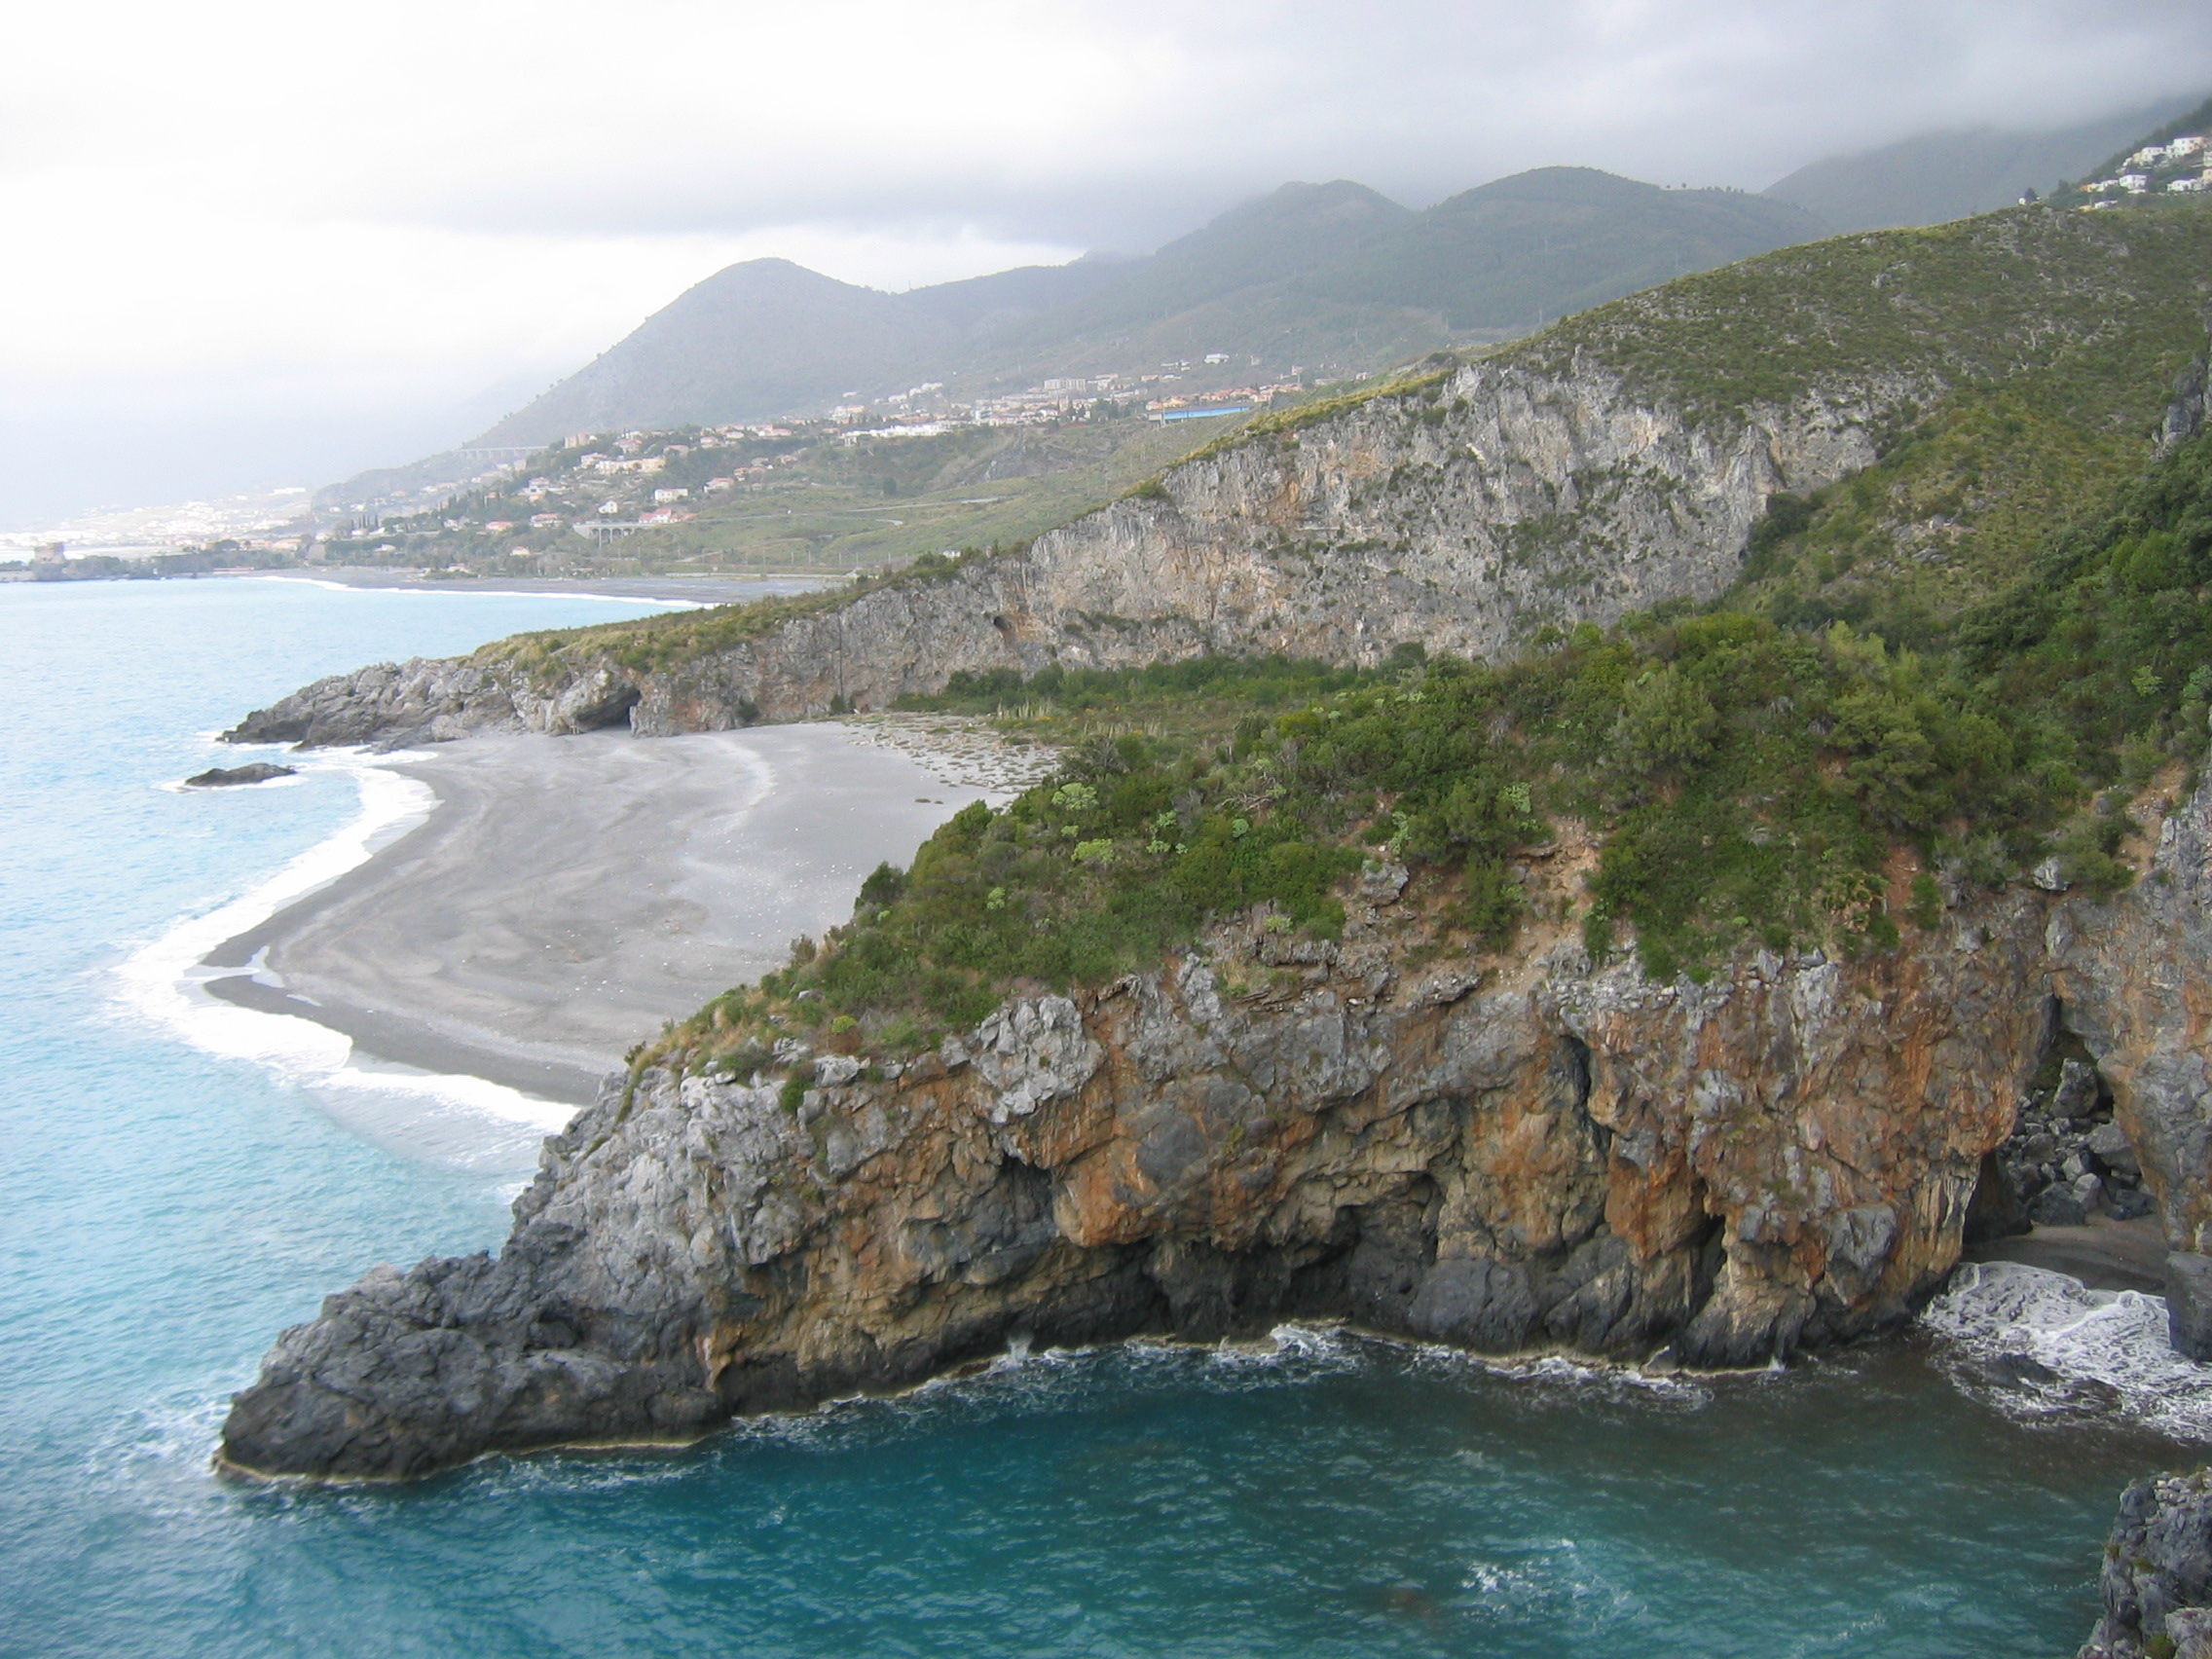
\includegraphics[width=\linewidth, height=0.25\paperheight]{../media/coastline}
	&\includegraphics[width=\linewidth, height=0.25\paperheight]{../media/bark}      &\\
	 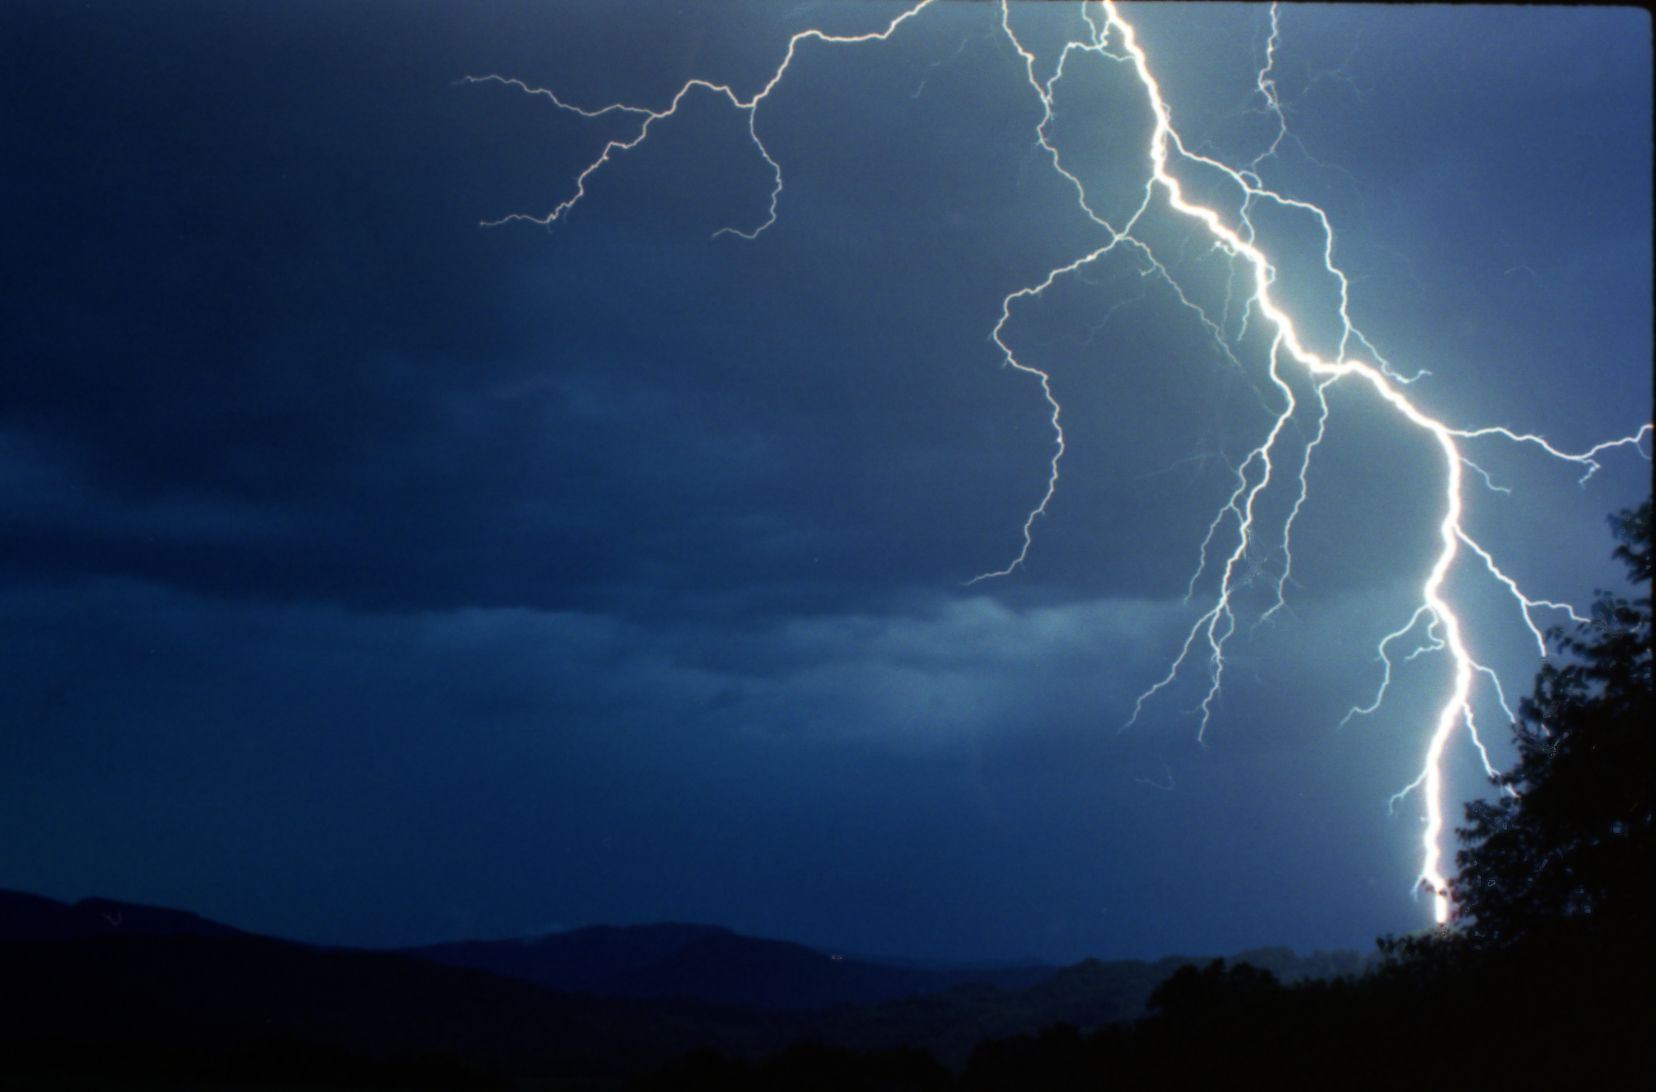
\includegraphics[width=\linewidth, height=0.25\paperheight]{../media/lightning}
	&Loads of real-life systems look rough or noisy; can we quantify, model or simulate this?
\end{tabular}
\end{frame}

\begin{frame}
\frametitle{Hard to describe a coastline}
\begin{columns}
\begin{column}{0.55\linewidth}
\vspace{1em}
\only<1>{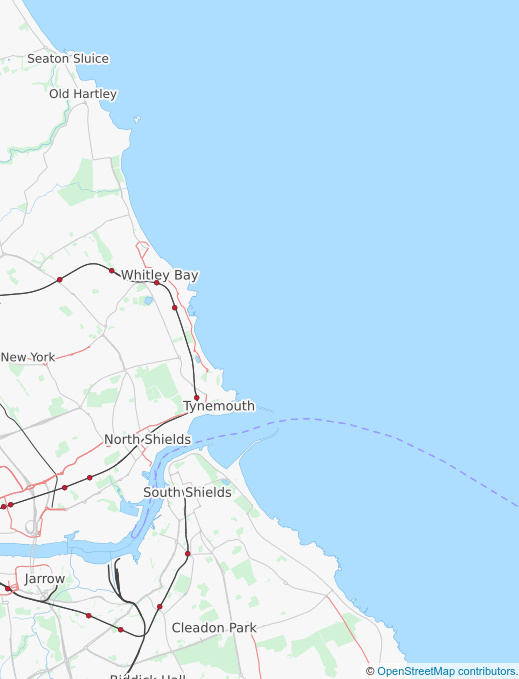
\includegraphics[width=\linewidth]{../media/processed/whitley_bay}}%
\only<2,3>{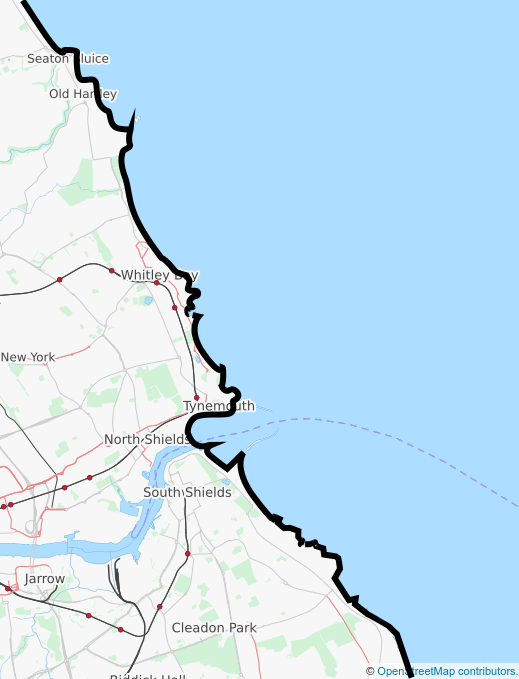
\includegraphics[width=\linewidth]{../media/processed/whitley_bay_boundary}}%
\only<4>{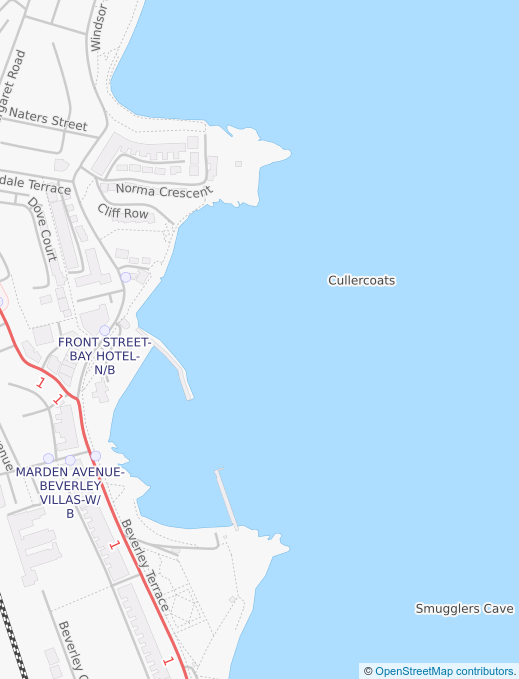
\includegraphics[width=\linewidth]{../media/processed/cullercoats}}%
\only<5>{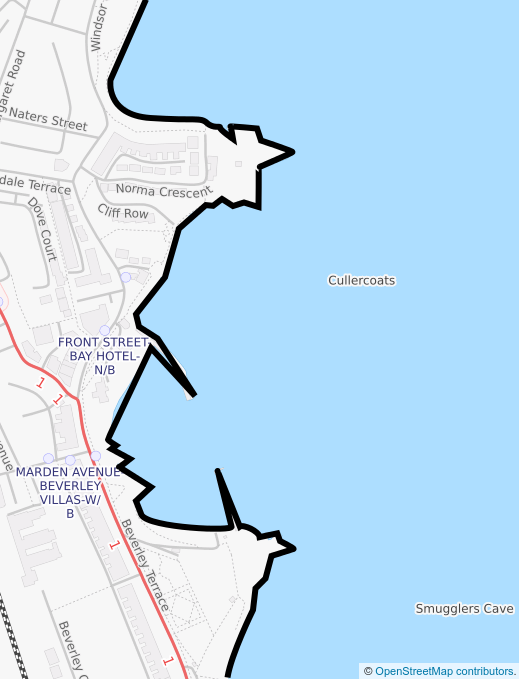
\includegraphics[width=\linewidth]{../media/processed/cullercoats_boundary}}%
\end{column}

\begin{column}{0.45\linewidth}
	Might want a differentiable (smooth) curve
	\begin{align*}
		f \colon [0, 1] &\to    \mathbb{R}^2 \\
		     t \enspace &\mapsto \begin{pmatrix}\,x(t) \\ \,y(t)\end{pmatrix}	
	\end{align*}
\pause
\begin{itemize}[<+->]
	\item Pain to write down
	\item Doesn't capture ``pointyness''
	\item Even more detail to describe when zoomed in
\end{itemize}
\end{column}

\end{columns}
\end{frame}

\foreach \name in {velcro, carrot_leaf, coffee_filter} {
	\picframe{../media/\name}{The world looks different when you change scale}
}

\begin{frame}
\frametitle{The world looks different when you change scale}
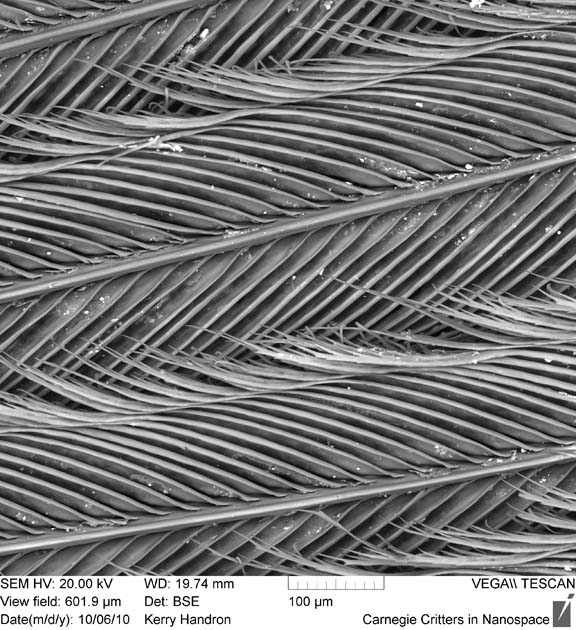
\includegraphics[width=0.33\linewidth]{../media/sem_feather}%
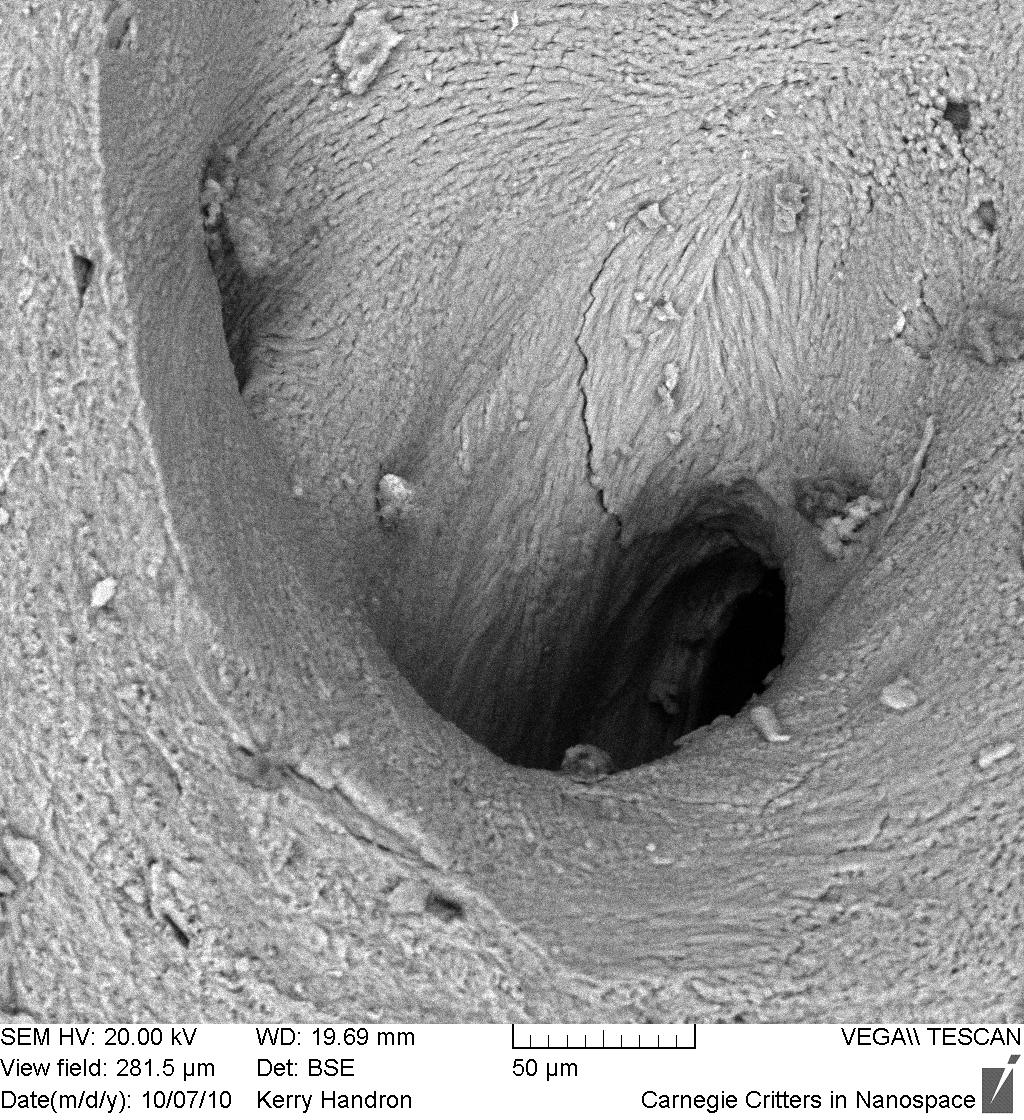
\includegraphics[width=0.33\linewidth]{../media/sem_bone}%
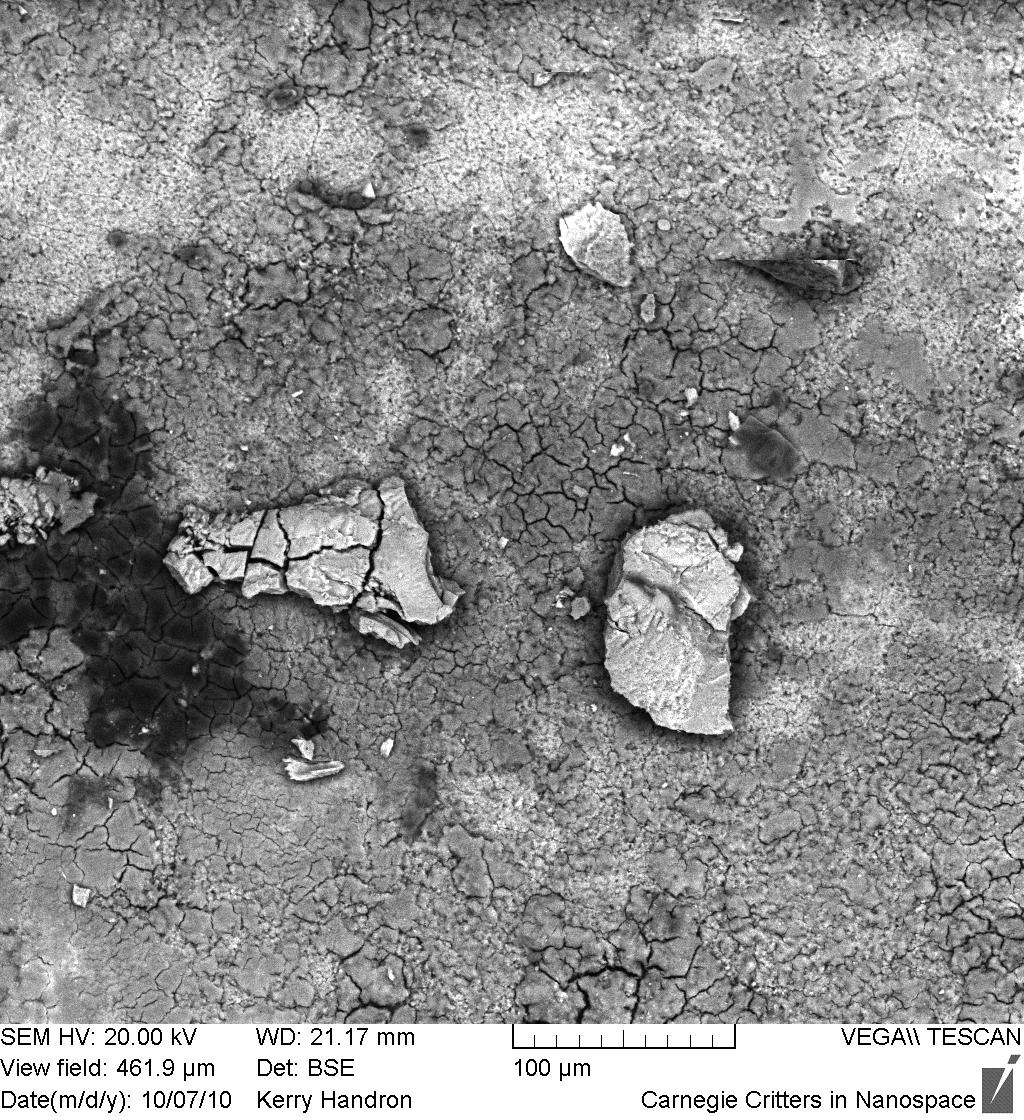
\includegraphics[width=0.33\linewidth]{../media/sem_egg}%
\pause

\hfil feather\pause\hfill bone\pause\hfill egg \hfil
\end{frame}

\begin{frame}
\frametitle{The world is different on different scales}
\hfill\alert{\Huge \dots Duh!}

\begin{center}
\begin{tabular}{lll}
	\toprule
	             Micro        &Meso             &Macro              \\
	\midrule
	\uncover<2->{Quantum      &Normal           &General Relativity}\\
	\uncover<3->{Observation  &Sample           &Population        }\\
	\uncover<4->{Time series  &Moving average   &Trend             }\\
	\bottomrule
\end{tabular}

\pause
\only<1-2>{%
	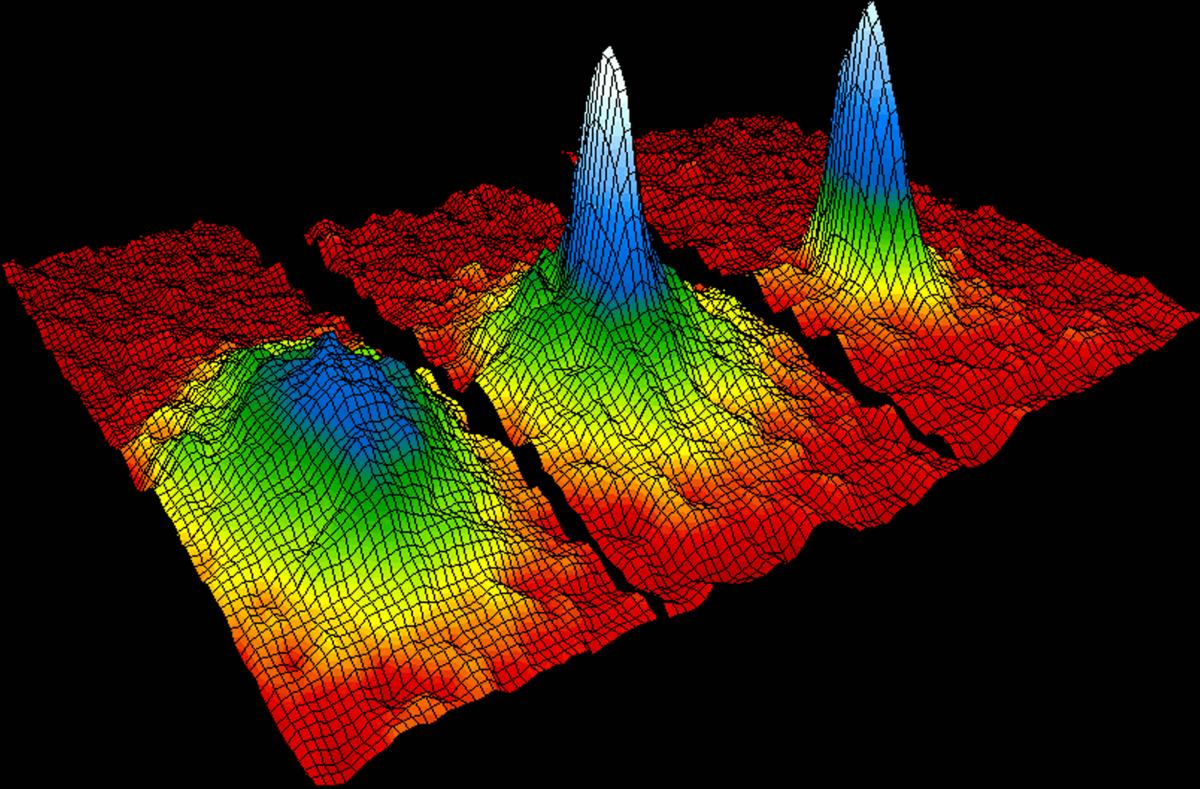
\includegraphics[height=0.3\textheight]{../media/bec}%
	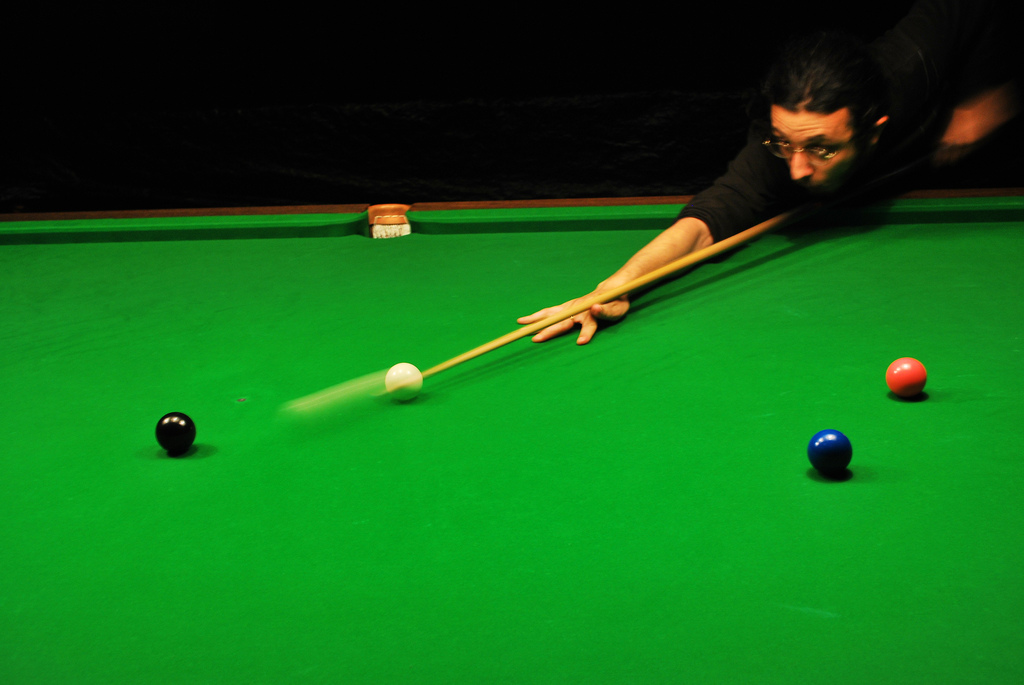
\includegraphics[height=0.3\textheight]{../media/snooker}%
	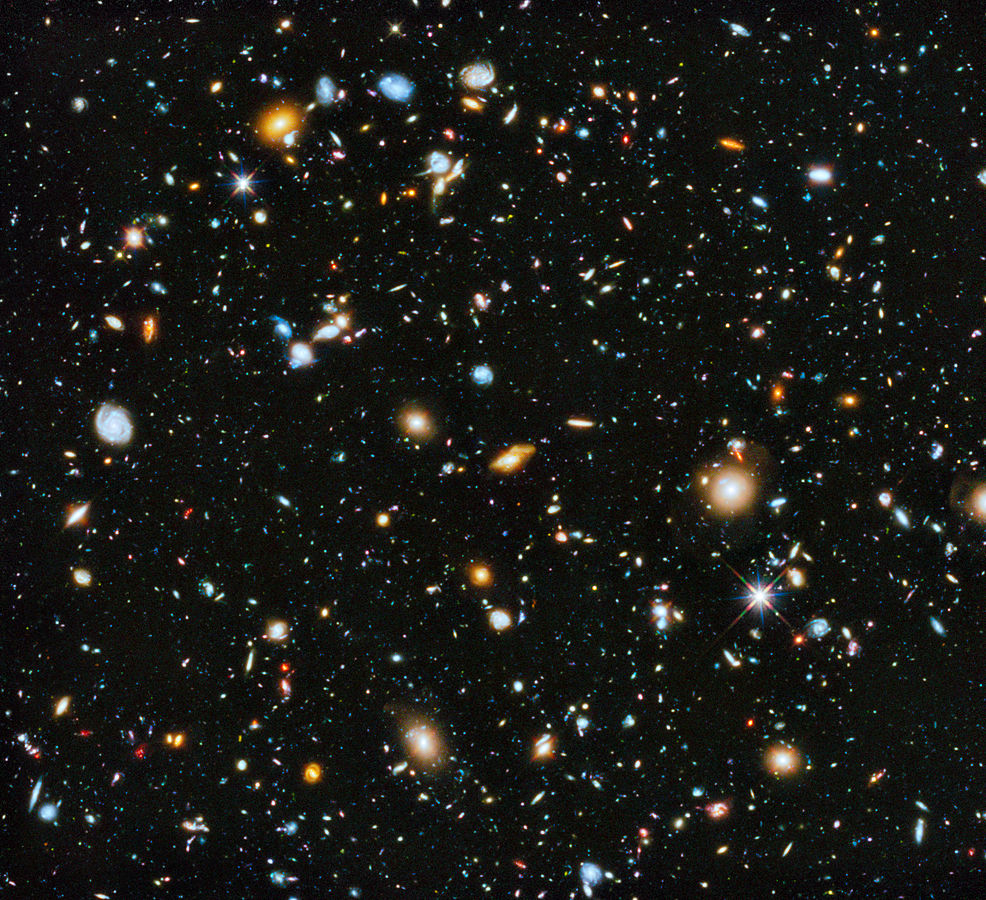
\includegraphics[height=0.3\textheight]{../media/universe}%
}%
\only<3>{%
	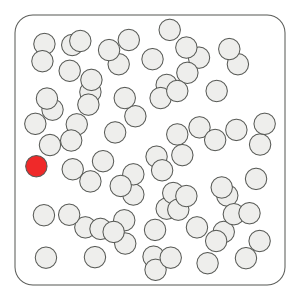
\includegraphics[height=0.3\textheight]{../media/processed/observation}%
	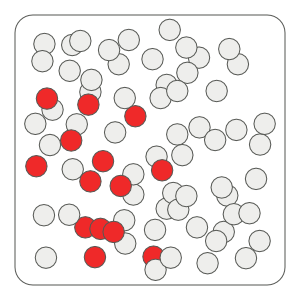
\includegraphics[height=0.3\textheight]{../media/processed/sample}%
	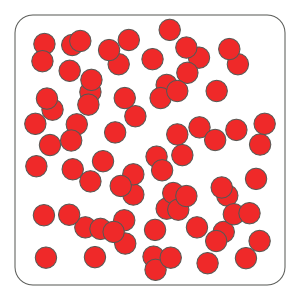
\includegraphics[height=0.3\textheight]{../media/processed/population}%
}%
\only<4>{%
	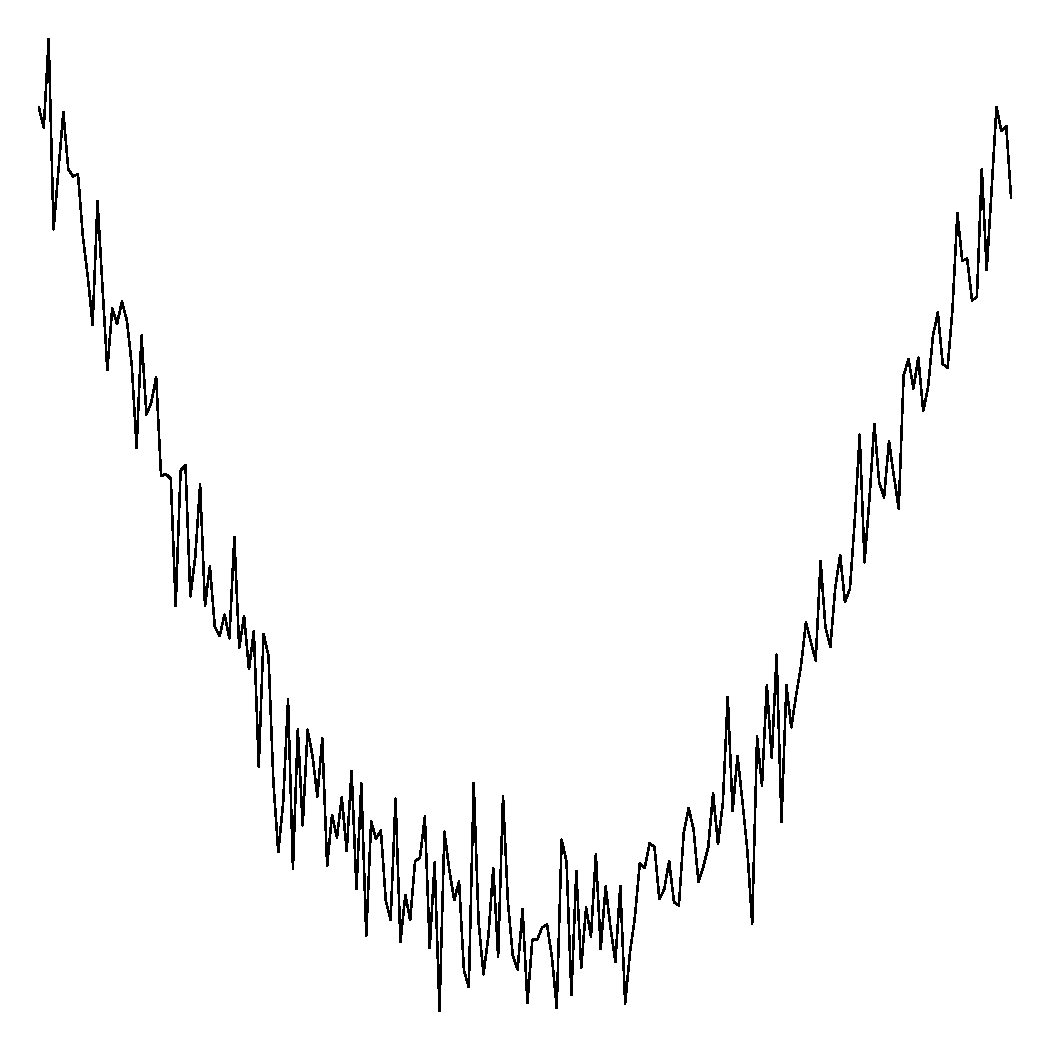
\includegraphics[height=0.3\textheight]{../media/processed/time_series}%
	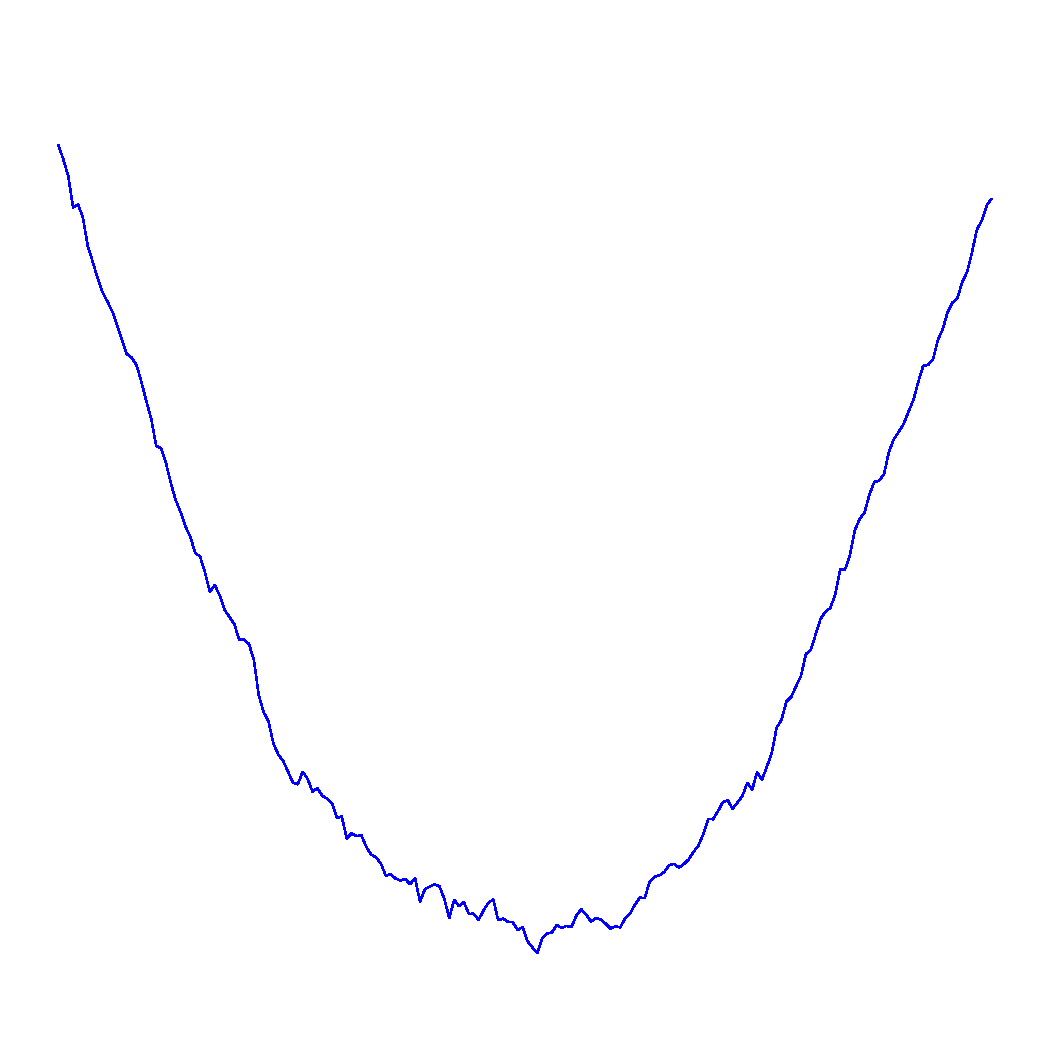
\includegraphics[height=0.3\textheight]{../media/processed/moving_average}%
	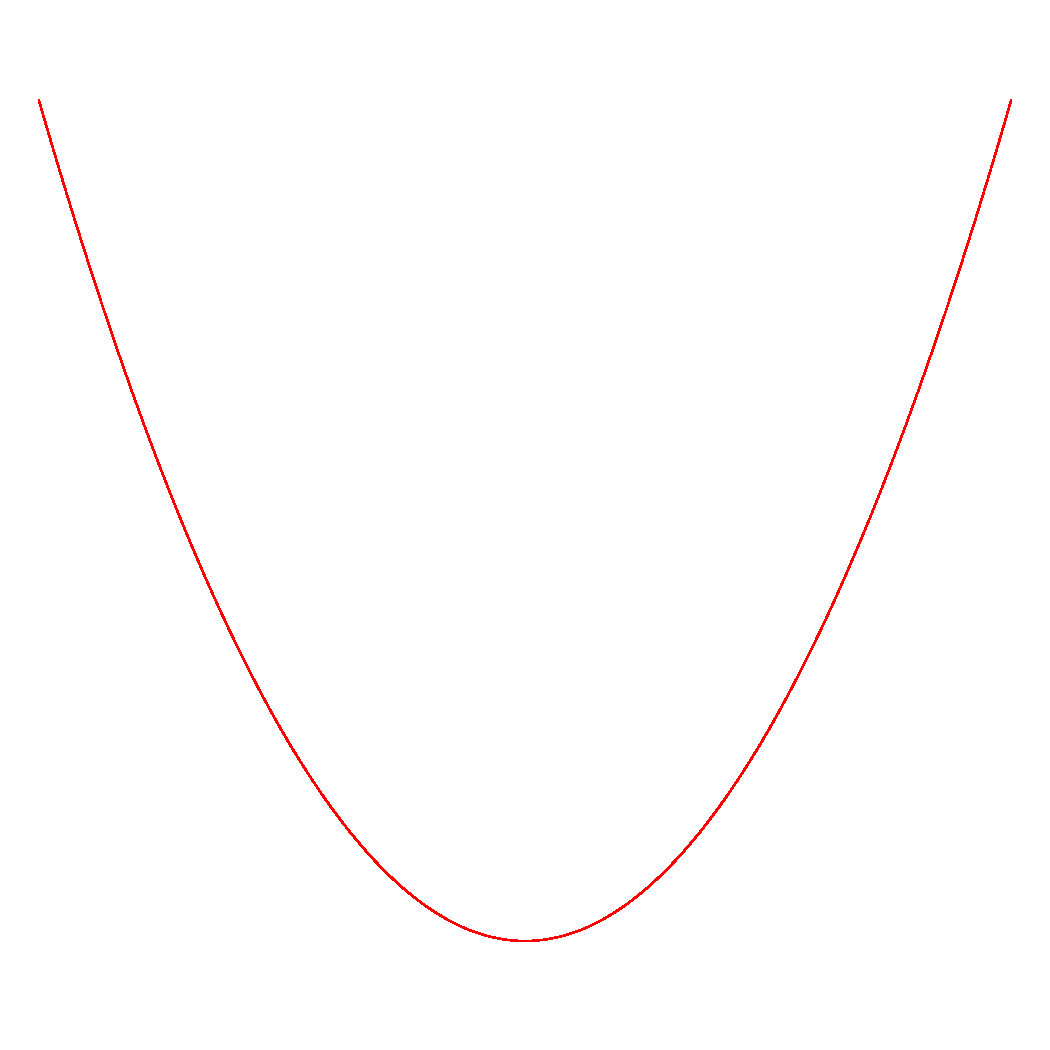
\includegraphics[height=0.3\textheight]{../media/processed/trend}%
}%
\end{center}
\end{frame}

\begin{frame}[standout]

{\Large Informal definition of a fractal:}
\begin{itemize}
	\item Geometric object \pause
	\item Self-similar  \pause
	\begin{itemize}
		\item exactly
		\item approximately
		\item statistically
	\end{itemize}  \pause
	\item Detailed at all scales
\end{itemize}
\end{frame}

\section{What: Mathematical description}

\begin{frame}
\frametitle{A definition}

\begin{definition}[Mandelbrot]
A \alert{fractal} is a subset $X \inside \reals^n$ whose Hausdorff dimension is strictly larger than its Lebesgue covering dimension.
\end{definition}

This relies upon a definition of \alert{dimension}.
\pause

Specifying ``dimension'' turns out to be tricky\dots
\end{frame}

\begin{frame}
\frametitle{Topological dimension \footnotesize\hfill also \emph{Lebesgue} or \emph{covering} dimension}
\begin{itemize}[<+->]
	\item \alert{Cover} of~$X$: a list of open sets $S_i$ with $X = S_1 \cup \dots \cup S_n$.
	\item Each point~$x$: count the number $N_S(x)$ of $T_i$ containing~$x$.
	\item Maximum such number $N_S$ is the \alert{order} of the cover.	
\end{itemize}

\begin{center}
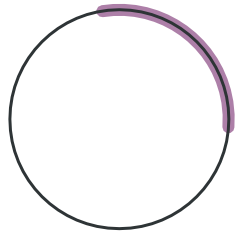
\includegraphics[width=0.25\linewidth]{../media/processed/covering_dimension1}
\quad
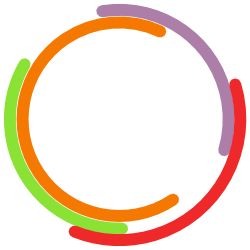
\includegraphics[width=0.25\linewidth]{../media/processed/covering_dimension2}
\quad
\onslide<4->{
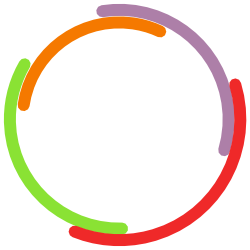
\includegraphics[width=0.25\linewidth]{../media/processed/covering_dimension3}
}
\end{center}

\begin{itemize}[<+->]
	\item \alert{Refine} the cover: break down the $S_i$ into smaller pieces.
	\item $\exists N:$ any cover can be refined to have order~$\leq N$.
	\item The \alert{topological dimension} of~$X$ is $\dimT(X) = N-1$.
\end{itemize}
\end{frame}

\begin{frame}
\frametitle{Box-counting dimension \footnotesize\hfill also \emph{Minkowski} dimension}

Say we're working with $X \subseteq \mathbb{R}^2$ and given some small $r > 0$.

\begin{itemize}
	\item How many $r \times r$ squares do you need to cover~$X$? \pause
	\item Call the number $N(r)$ and $N(\sfrac 1 1), N(\sfrac 1 2), N(\sfrac 1 3), N(\sfrac 1 4), \dotsc$. 	\pause
	\item \alert{Example:} if $X = \text{unit square}$ then $N(1/n) = n^2$. 
\end{itemize}
\begin{center}
	
\includegraphics[width=\linewidth]{../media/processed/box_counting}
\end{center}	
	\hfill $1 = 1^2$
	\hfill\hfill $2^2 = 4$
	\hfill\hfill $3^3 = 9$
	\hfill\hfill $4^2 = 16$
	\hfill{}
\pause
\begin{align*}
	N = (1/n)^2 = r^{-2} &\iff \log N = -2 \log(r) \\&\iff \log N / -\log(r) = 2
\end{align*}
\end{frame}

\begin{frame}
\frametitle{Box-counting dimension \footnotesize\hfill also \emph{Minkowski} dimension}
\alert{Example:}	 $X = \text{Great Britain's coastline}$
\begin{center}
	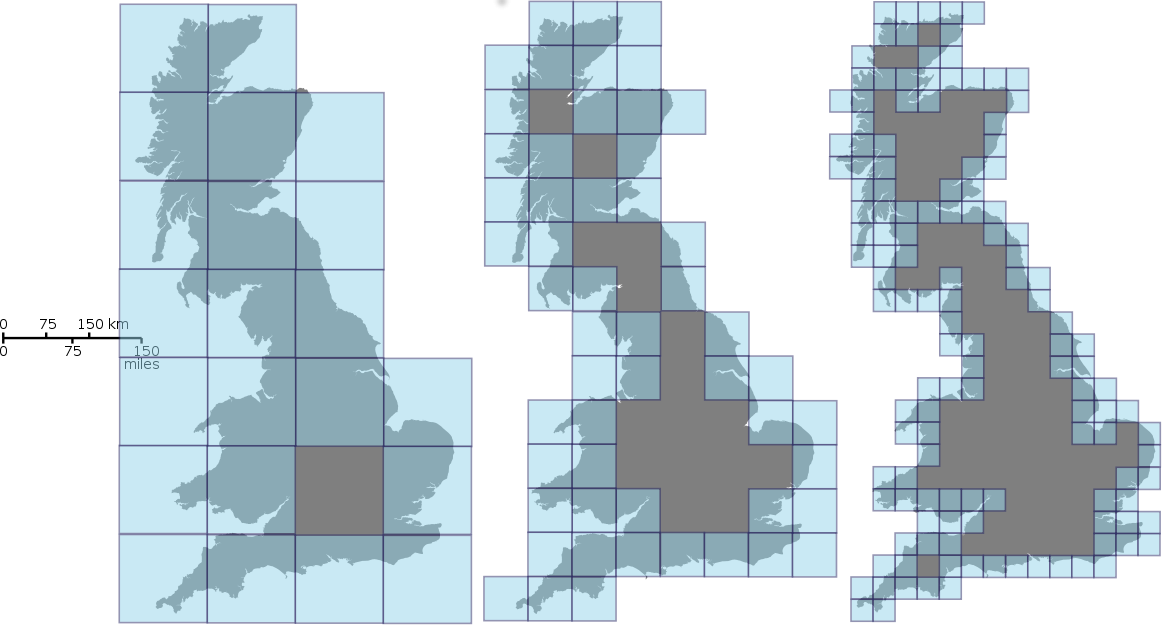
\includegraphics[width=0.9\linewidth]{../media/box_dimension}
\end{center}
\pause
Dimension defined by $\displaystyle \dimB(X) = \lim_{r \to 0} \frac{N(r)}{-\log(r)} \approx 1.25 \color{red}\notin \mathbb{Z}\,!!$.
\end{frame}

\begin{frame}
\frametitle{Too many dimensions}
The ``official'' fractal dimension is the \alert{Hausdorff dimension}
\pause
\begin{itemize}[<+->]
	\item Nice special case: \alert{similarity dimension} (coming shortly)
\end{itemize}
\pause[\thebeamerpauses]
There are loads more to choose from.
Choose the right tool for the job!
\pause
\begin{itemize}
	\item information dimension
	\item correlation dimension
	\item Assouad dimension
	\item packing dimension
	\item \dots	
\end{itemize}
\end{frame}

\section{HOW: Mathematical models}

\begin{frame}
\frametitle{A recipe for making fractals}
\begin{itemize}
	\item Need detail at all levels \& self-similarity
	\item To achieve this: often the limit of a recursive construction
\end{itemize}
\pause
One recipe (of many): \alert{teragons}
\medskip
\begin{columns}
\begin{column}{0.6\linewidth}
\begin{itemize}[<+->]
	\item \alert{Initial setup:} a line segment
	\item Replace with a scaled \& rotated copy of the \alert{generator}
	\item Do the same to the new subsegments
	\item Repeat until bored
\end{itemize}
\end{column}
\begin{column}{0.4\linewidth}
\centering
\bigskip
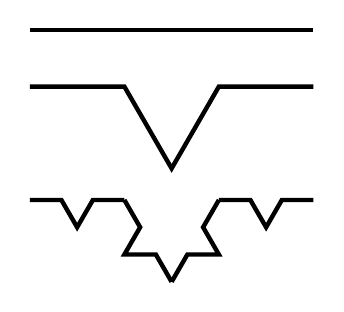
\begin{tikzpicture}[xscale=1.2, yscale=-1.2]
	\draw[ultra thick, visible on=<2->] (0, 0) -- (3, 0);
	\tikzset{yshift=0.6cm}
	\draw[ultra thick, visible on=<3->] (0, 0) \kochsegment{0}{1};
	\tikzset{yshift=1.2cm}
	\draw[ultra thick, visible on=<4->, alert on=<4>] (0, 0) \kochsegment{0}{1/3};
	\draw[ultra thick, visible on=<5->, alert on=<5>] (1, 0) \kochsegment{60}{1/3};
	\draw[ultra thick, visible on=<6->, alert on=<6>] (1, 0) ++ (60:1) \kochsegment{-60}{1/3};
	\draw[ultra thick, visible on=<7->, alert on=<7>] (2, 0) \kochsegment{0}{1/3};
\end{tikzpicture}
\onslide<8->{\includegraphics{tikz/koch_3}}
\end{column}
\end{columns}
\end{frame}

\begin{frame}[standout]
\frametitle{\mbox{\Large Limit called the \emph{Koch curve}}}%
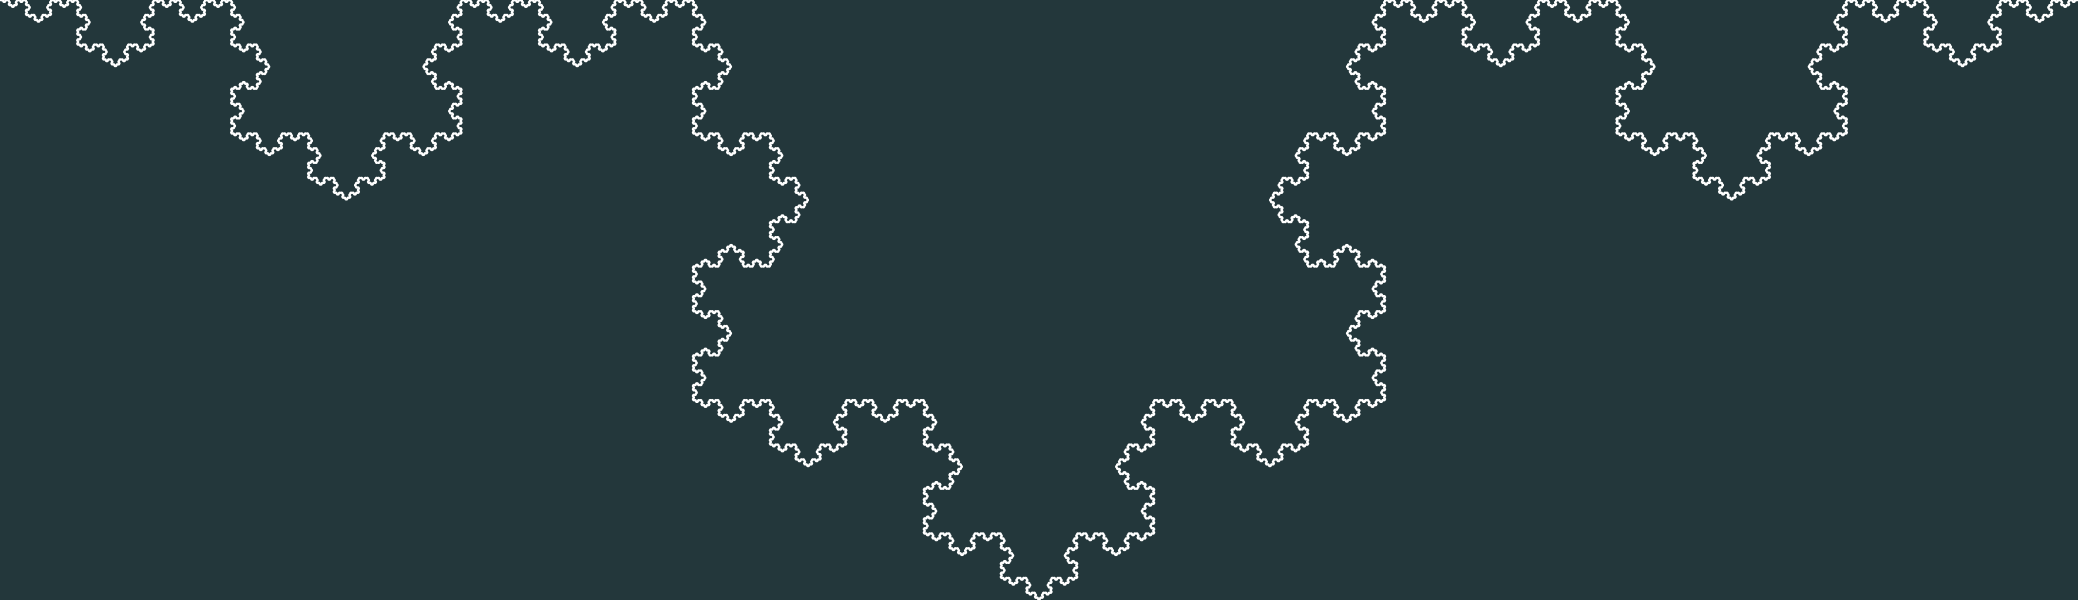
\includegraphics[width=\linewidth]{../media/renders/koch_curve}
\pause
\begin{itemize}[<+->]
	\item[] Infinite length \quad\enspace\qquad $(\sfrac 4 3)^n \to \infty$
	\item[] Encloses finite area	
	\item[] Topological dimension \enspace $1$
	\item[] Fractal dimension $\log(4)/\log(3) \approx 1.262$
\end{itemize}
\end{frame}

\definecolor{highlight1}{HTML}{EF2929}
\definecolor{highlight2}{HTML}{FACF3E}
\definecolor{highlight3}{HTML}{8Ae234}
\definecolor{highlight4}{HTML}{729FCF}

\begin{frame}[standout]
\frametitle{\mbox{\Large Similarity dimension}}%
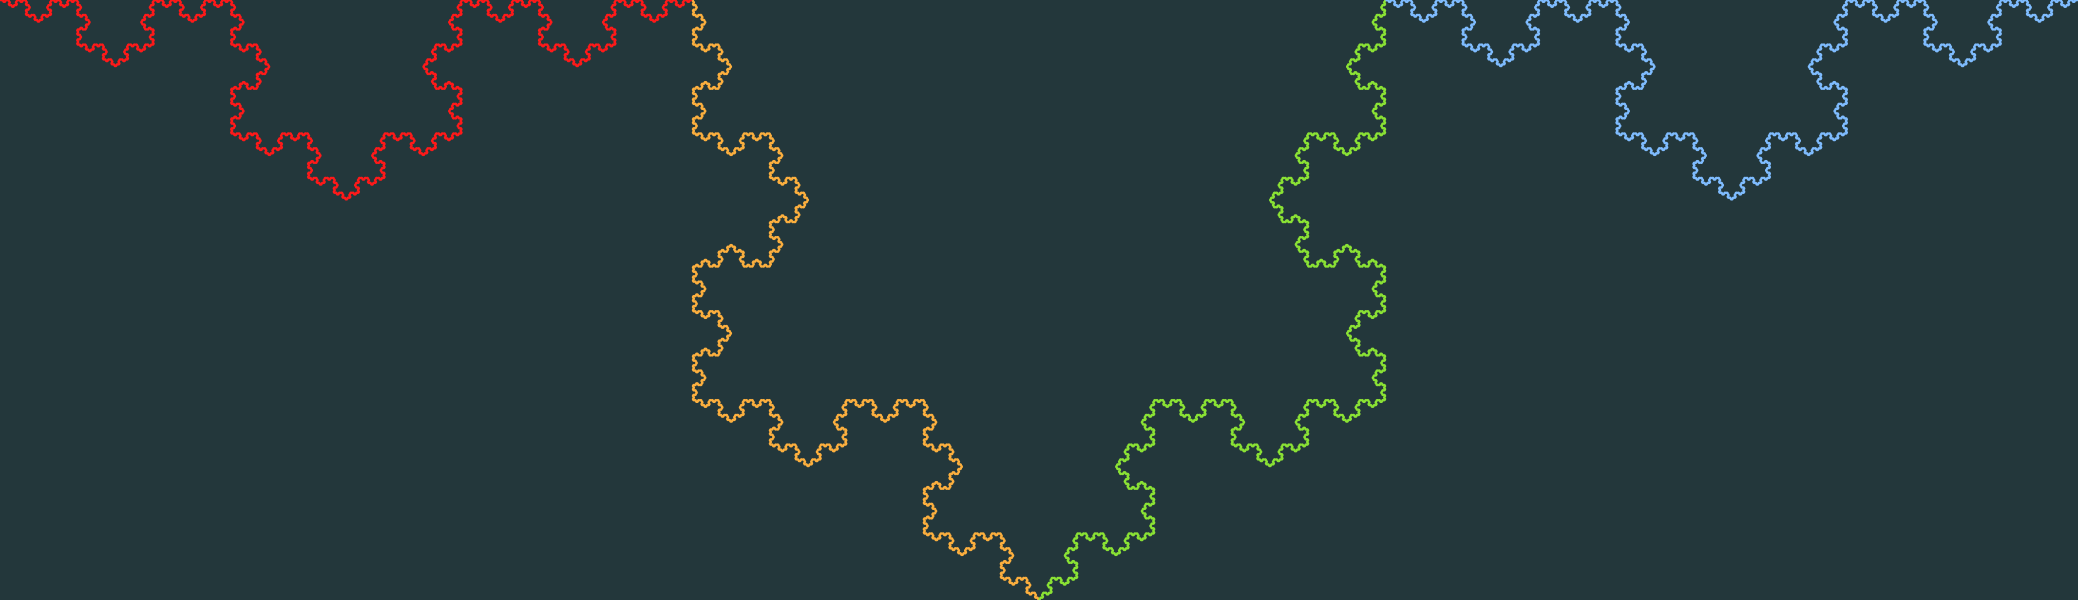
\includegraphics[width=\linewidth]{../media/renders/koch_similarity}
\pause \mdseries
\begin{itemize}[<+->]
	\item $\displaystyle K =
       {\color{highlight1!90!white}K_1}
\sqcup {\color{highlight2}K_2}
\sqcup {\color{highlight3}K_3}
\sqcup {\color{highlight4!95!white}K_4}$
	\item Fractal $=4$ copies of itself at $1/3$ scale
	\item Solve $\sfrac 1 3^d + \sfrac 1 3^d + \sfrac 1 3^d + \sfrac 1 3^d = 1$
	\item $\dimS = \log 4 / \log 3$
\end{itemize}
\end{frame}

\begin{frame}
\frametitle{Similarity dimension in general}
{\Large
\begin{equation*}
	K = K_1 \sqcup K_2 \sqcup \dots \sqcup K_n
\end{equation*}
}
\pause
\begin{itemize}[<+->]
	\item Each copy~$K_i$ is a scaled copy of~$K$ {\small\hfill(say at scale $r_i < 1$)}
	\item Solve $r_1^d + \dots + r_n^d = 1$       {\small\hfill(e.g.\ numerically)}
	\item $\dimS$ is the unique solution~$d$
\end{itemize}
\end{frame}
\end{document}